\documentclass[12pt]{exam}
\usepackage[utf8]{inputenc}
\usepackage{graphicx,lastpage}

\usepackage[margin=0.5in]{geometry}
\usepackage{amsmath,amssymb}
\usepackage{multicol}
\usepackage{verbatim}
\usepackage{listings}

\newcommand{\class}{Math I}
\newcommand{\term}{Winter 2014}
\newcommand{\examnum}{Exam 1}
\newcommand{\examdate}{1/11/2016}
\newcommand{\timelimit}{75 Minutes}


\pagestyle{head}
\firstpageheader{}{}{}
\runningheader{Winter Workshop Test}{ Page \thepage\ of \numpages}{\examdate}
\runningheadrule


\begin{document}

\begin{center}

\includegraphics[scale=0.25]{logo.png}\\
\vspace{2mm}
in assocation with\\


\includegraphics[scale=0.75]{Selection_002.png}
\vspace{2mm}



\noindent
\textbf{Winter Workshop Test}

\begin{tabular*}{\textwidth}{l @{\extracolsep{\fill}} c r @{\extracolsep{6pt}} l}
\textbf{Date:1/11/2016} & \textbf{Maximum Marks:25+30+15=70}& \textbf{Time: 60 minutes} & \\ %\makebox[2in]{\hrulefill}\\
%\textbf{\term} &&\\
%\textbf{\examnum} &&\\
%\textbf{\examdate} &&\\
%\textbf{Time Limit: \timelimit} & Teaching Assistant & \makebox[2in]{\hrulefill}
\end{tabular*}\\
\rule[2ex]{\textwidth}{2pt}


\textbf{General Instructions}
\begin{enumerate}
\item This exam consists of three sections:
\begin{itemize}
\item Logical Resoning
\item KRAIG
\item Programming
\end{itemize} 
\item The third section is optional. It is to be attempted by those who would like to take part in the Image Processing workshop
\item Make sure all the information below is filled up
\end{enumerate}
\end{center}

\raggedright
\textbf{Name:} \makebox[6.5in]{\hrulefill}\\
\textbf{Roll No.:} \makebox[2in]{\hrulefill}\hspace{1cm}\textbf{Hall:}\makebox[2cm]{\hrulefill} \hspace{1cm}\textbf{Contact:}\makebox[1.5in]{\hrulefill}\\

\vspace{5mm}
Which Workshop are you planning to do? Autonomous \fbox{
	\begin{minipage}{3mm}
		\hfill\vspace{3mm}
	\end{minipage}
	} Image Processing \fbox{
	\begin{minipage}{3mm}
		\hfill\vspace{3mm}
	\end{minipage}
	}
	\vspace{1mm}
\\Prior Knowledge in Programming? Yes \fbox{
	\begin{minipage}{3mm}
		\hfill\vspace{3mm}
	\end{minipage}
	} No\fbox{
	\begin{minipage}{3mm}
		\hfill\vspace{3mm}
	\end{minipage}
	}\vspace{1mm}
\\What is your EAA? NSO \fbox{
	\begin{minipage}{2.6mm}
		\hfill\vspace{2.6mm}
	\end{minipage}
	} NCC \fbox{
	\begin{minipage}{2.6mm}
		\hfill\vspace{2.6mm}
	\end{minipage}
	} NSS \fbox{
	\begin{minipage}{2.6mm}
		\hfill\vspace{2.6mm}
	\end{minipage}
	}\vspace{1mm}
\\Which Phase will you attend? $1^{st} Dec - 7^{th} Dec$ \fbox{
	\begin{minipage}{3mm}
		\hfill\vspace{3mm}
	\end{minipage}
	} $10^{st} Dec - 16^{th} Dec$ \fbox{
	\begin{minipage}{3mm}
		\hfill\vspace{3mm}
	\end{minipage}
	}


\begin{center}
\textbf{For official use only}\\
\addpoints
\begin{tabular}{|l|c|c|c|c|}
\hline
Section & 1 & 2 & 3 & Total\\
\hline
Marks & & & &\\
\hline
\end{tabular}
%\gradetable[h][questions]
\vspace{5mm}
\\Corrected By: \makebox[2in]{\hrulefill}
\end{center}


\noindent
\rule[2ex]{\textwidth}{2pt}

\centering \large \textbf{LOGICAL REASONING}

\normalsize

\begin{questions}



\question[2] Before Mt. Everest was discovered, what was the tallest mountain in the world?.
\vspace{5mm}
\\
\makebox[7in]{\hrulefill}
\addpoints

\question[2] Which word in the dictionary is spelled incorrectly?
\vspace{5mm}
\\
\makebox[7in]{\hrulefill}
\addpoints

\question[2] Tickets numbered 1 to 20 are mixed up and then a ticket is drawn at random. What is the probability that the ticket drawn has a number which is a multiple of 3 or 5? \hfill \fbox{
	\begin{minipage}{1cm}
		\hfill\vspace{3mm}
	\end{minipage}
	}
\addpoints

\question[4]Adam, Bob, Clair and Dave are out walking: They come to rickety old wooden bridge. The bridge is weak and only able to carry the weight of two of them at a time. Because they are in a rush and the light is fading they must cross in the minimum time possible and must carry a torch (flashlight) on each crossing.\\

They only have one torch and it can't be thrown. Because of their different fitness levels and some minor injuries they can all cross at different speeds. Adam can cross in 1 minute, Bob in 2 minutes, Clair in 5 minutes and Dave in 10 minutes.\\

Adam, the brains of the group thinks for a moment and declares that the crossing can be completed in 17 minutes. There is no trick. How is this done?
\fillwithlines{8em}
\addpoints

\question[3]
Fernando Alonso and Sebastian Vettel go for a car race. Before start of race, both of them have the exactly same amount of fuel in their respective cars. With the given fuel Fernando can drive continuously for 4 hours while Vettel can drive 1 hour more i.e five hours.After a time they realize that amount of fuel left in Sebastian car is 4 times the fuel in Fernando car.For how long they are racing ?
\hfill \fbox{
	\begin{minipage}{1cm}
		\hfill\vspace{3mm}
	\end{minipage}
	}
\addpoints

\question[5]
A man desired to get into his work building, however he had forgotten his code. 
However, he did recollect five pieces of information
\begin{enumerate}
\item Sum of 5th number and 3rd number is 14.
\item Difference of 4th and 2nd number is 1.
\item The 1st number is one less than twice the 2nd number.
\item The 2nd number and the 3rd number equals 10.
\item The sum of all digits is 30.
\end{enumerate}

Crack the code ?\hfill \fbox{
	\begin{minipage}{1.5cm}
		\hfill\vspace{3mm}
	\end{minipage}
	}

\addpoints

\question[4]
Two women play a dice game where two standard dice are rolled. Woman A says that a 11 will be rolled first. Woman B says that two consecutive 8s will be rolled first. The women keep rolling until one of them wins.


What is the probability that A will win ?
\hfill \fbox{
	\begin{minipage}{1cm}
		\hfill\vspace{3mm}
	\end{minipage}
	} 
\addpoints

\question[5]
Eight family members A, B, C, D, E, F, G and H are sitting around a circular table but not necessarily in the same order. Some of them are females and some of them are males. All of them are related to each other in the same way or the other. Some of them are facing the centre while some are facing outside.
\begin{enumerate}

\item[-] Only two people sit between B and E, B faces the centre. F sits second to the right of B. E is the wife of A. No female is an intermediate neighbour of E.
\item[-] C is not an immediate neighbour of B. C is the daughter of E. Both the immediate neighbours of C face the centre. Only three people sit between A and C’s brother. F is not the brother of C. Neither A nor C’s brother is an immediate neighbour of F.
\item[-] H, wife of B sits to the immediate left of D. Both G and A face a direction opposite to that of C. C’s husband sits second to the left of G. B’s father sits to the immediate right of E.B sits second to the right of F.


\end{enumerate}
\begin{enumerate}
\item Who among the following faces outside the centre ?
\begin{multicols}{2}
\begin{choices}
\choice C and F
\choice F and G
\choice G and H
\choice A and G

\end{choices}
\end{multicols}
\item Who among the following is brother of C ?
\begin{multicols}{2}
\begin{choices}
\choice 	A
\choice D
\choice B
\choice H
\addpoints

\end{choices}
\end{multicols}
\end{enumerate} 
\end{questions}
\rule[2ex]{\textwidth}{2pt}
\centering \textbf{Space for Rough Work}
\newpage
\centering \large \textbf{KRAIG}
\normalsize
\begin{questions}

\question[2]Write the full-forms of:
\begin{enumerate}
\item PWM:   \makebox[5in]{\hrulefill}
\item OpAmp: \makebox[5in]{\hrulefill}
\item IC: \makebox[5in]{\hrulefill}
\item RPM: \makebox[5in]{\hrulefill}
\end{enumerate}

\question[3] Write True or False:
\begin{enumerate}

\item An Ackerman Drive bot can move in any direction by changing its orientation:
\item  Zener diodes conduct in Forward Bias: 
\item  Scissor lift mechanism is used for cutting:
\item  OpAmps can be used as Comparators:
\item  IR photodiodes don’t become conducting when exposed to sunlight:
\item If a DC motor is connected to an AC source, it will periodically change direction of rotation:
\end{enumerate}

\question[10] Select the correct option. (More than one may be correct):
\begin{enumerate}
\item[i.] Which is the anode of an LED:\\
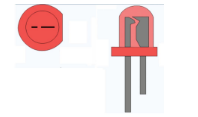
\includegraphics[scale=1]{LED.png}

\begin{choices}
\choice 	The longer terminal
\choice The shorter terminal
\choice The terminal on the side which has a cut in the bulb
\choice  The terminal which is on the side of the bulb without a cut
\addpoints

\end{choices}
\item[ii.] Relays are useful because:
\begin{choices}
\choice They can keep the user safe from shock.
\choice They are quickest available electronically operated switches.
\choice They are cheap.
\choice All of the above.
\end{choices}




\item[iii.]   Regarding motor driver L293D which of the following are correct?
\begin{choices}
\choice If Enable pins are LOW the motors are in free run.
\choice  If Enable pins are LOW the motors are in breaking condition.
\choice  If En1 pin is HIGH, and In1 and In2 pins are LOW, motor is in breaking condition.
\choice  If En1 pin is HIGH, and In1 and In2 pins are HIGH, motor is in breaking condition.
\end{choices}
\newpage

\item[iv.] Diodes are	:
\begin{choices}
\choice  Bi-directional switches.
\choice Conductors when N-side is connected to anode and P-side to cathode.
\choice Used in voltage regulation circuits.
\choice All of the above.
\end{choices}

\item[v.]  What are pins 4 and 5, and 12 and 13 of the L293D used for?
\begin{multicols}{2}
\begin{choices}
\choice Ground
\choice Heat sink
\choice Input
\choice Output
\end{choices}
\end{multicols}
\end{enumerate}

\question[5] Select the correct option (Single-correct type question):
\begin{enumerate}
\item[i.] If a pulsating signal is high for 0.3 ms and off for 0.1 ms in a cycle, what is the frequency and duty cycle of it?
\begin{multicols}{2}
\begin{choices}
\choice 33.33 ; 66.67\% 
\choice 25 ; 75\%
\choice 33.33 ; 75\%
\choice 25 ; 66.67\%
\end{choices}
\end{multicols}

\item[ii.]What voltage will an ac voltmeter display?
\begin{multicols}{2}
\begin{choices}
\choice RMS
\choice Peak Value
\choice Average
\choice Peak-to-peak value
\end{choices}
\end{multicols}

\item[iii.]What is the Pin No. 8 on an L293D used for?
\begin{multicols}{2}
\begin{choices}
\choice Enable
\choice Vcc
\choice Supply Voltage
\choice GND
\end{choices}
\end{multicols}

\item[iv.]What are the effects of moving a closed wire loop through a magnetic field?

\begin{choices}
\choice  A voltage is induced in the wire
\choice A current is induced in the wire 
\choice The polarity across the wire depends on the direction of motion
\choice All of the above
\end{choices}

\item[v.]In a factory where there are flammable fluids stored, which types of switches are most likely to be used in the storage rooms?
\begin{multicols}{2}
\begin{choices}
\choice Transistors
\choice Relays 
\choice SPSTs 
\choice All of the above
\end{choices}
\end{multicols}

\end{enumerate}

\question[5] Design a control circuit for a differential drive with 2 motors, using relay switches.
\end{questions}
\newpage

\centering \large \textbf{Programming}
\normalsize
\begin{questions}


\question[1]What is the output of the following code?
\begin{lstlisting}
#include <stdio.h>
int main() {
	int i = 2;
	printf("%d %d\n", ++i, i++);
	return 0;
}
\end{lstlisting}
\begin{multicols}{2}
\begin{choices}	
\choice 2 4
\choice 3 4
\choice 3 3
\choice 2 2
\end{choices}
\end{multicols}

\question[1] Which of the data types can overflow? Multiple can be correct
\begin{multicols}{2}
\begin{choices}	
\choice int
\choice float
\choice unsigned int
\choice double
\end{choices}
\end{multicols}

\question[1] Let’s say you want to calculate distance between the points (x1, y1) and (x2, y2). Which is a more appropriate expression?
\begin{choices}	
\choice  sqrt(pow((x2 - x1), 2) + pow(y2 - y1, 2)))

\choice  (y2 - y1) * sqrt(pow((x2 - x1)/(y2 - y1), 2)+1)

\end{choices}

\question[1]  Is this code valid?
\begin{lstlisting}
#include <stdio.h>
int main() {
	int a = 2, b = 3;
const int *p = &a;
p = &b;
return 0;
} 
\end{lstlisting}
\fbox{
	\begin{minipage}{1.5cm}
		\hfill\vspace{3mm}
	\end{minipage}
	}

\question[1]What is the output of the following code?
\begin{lstlisting}
#include <stdio.h>
int main() {
	int i = 2;
	printf("%d %d\n", ++i, i++);
	return 0;
}
\end{lstlisting}
\begin{multicols}{2}
\begin{choices}	
\choice 2 4
\choice 3 4
\choice 3 3
\choice 2 2
\end{choices}
\end{multicols}

\question[2]Which is a valid representation of a string? Multiple can be correct.
\begin{choices}	
\choice char str[5] = \{'a', 'b', 'c', 'd', 'e' \};
\choice char str[5] = \{'a', 'b', 'c', 'd', 'e', '\textbackslash 0'\};
\choice char str[5] = \{'\textbackslash0', 'a'\};
\choice char str[5] = \{'a', 'b', 'c', 'd', '\textbackslash 0'\};
\choice char str[5] = \{'a', 'b', 'd', '\textbackslash 0'\};
\end{choices}

\question[2]How would you swap the value of two integers a and b without using a temporary variable?
\makeemptybox{5em}

\question[2]What is the difference between `char *a` and `char a[ ]?
\makeemptybox{5em}
\question[2]Write only the for loops for printing this sequence:\\
1\\
12\\
123\\
1234\\
12345\\
1234\\
123\\
12\\
1 
\makeemptybox{6em}


\question[2] Output of the following code will be:
\begin{lstlisting}
main()
	{
	int i=-1,j=-1,k=0,l=2,m;
	m=i++ && j++ && k++ || l++;
	printf(“%d %d %d %d %d”, i,j,k,l,m);
	}
\end{lstlisting}
\begin{multicols}{2}
\begin{choices}	
\choice 0 0 1 3 1
\choice -1 -1 0 2 1	
\choice -1 -1 0 2 0
\choice -1 0 0 2 1
\end{choices}
\end{multicols}




\end{questions}
\begin{comment}
\begin{questions}
\question[20] Consider the function $f(x)=3x^3+2x^2+x+1$.
\noaddpoints % to omit double points count
\begin{parts}
\part[10] Calculate $f'(x)$.
\part[10] Calculate $f''(x)$.
\end{parts}
\addpoints

\question[2] One of these things is not like the others; one of these
things is not the same. Which one is different?
\begin{choices}
\choice John
\choice Paul
\choice George
\choice Ringo
\choice Socrates
\end{choices}

\question[2] One of these things is not like the others; one of these
things is not the same. Which one is different?
\begin{oneparchoices}
\choice John
\choice Paul
\choice George
\choice Ringo
\choice Socrates
\end{oneparchoices}

\question[3] Mark box if true.
\addpoints
\begin{checkboxes}
\choice 2+2=4
\choice $\frac{d}{dx} (x^2+1) = 2x+1$
\choice The Moon is made of cheese.
\end{checkboxes}

{%
\checkboxchar{$\Box$} % changing checkbox style locally
\question[3] Mark box if true.
\addpoints
\begin{checkboxes}
\choice 2+2=4
\choice $\frac{d}{dx} (x^2+1) = 2x+1$
\choice The Moon is made of cheese.
\end{checkboxes}
}%

{%
% changing choice items style locally
\renewcommand*\thechoice{\arabic{choice}} 
\renewcommand*\choicelabel{\thechoice)}
%
\question[2] Element with $Z=92$ is:
\begin{multicols}{2}
\begin{choices}
\choice H
\choice O
\choice F
\choice S
\choice Ba
\choice Pb
\choice U
\choice Pu
\end{choices}
\end{multicols}
}%

\question[10]
In no more than one paragraph, explain why the earth is round.
\makeemptybox{2in}

\question[20]
Explain blah, blah\ldots
\makeemptybox{\fill}

\newpage

\question[20]
Explain blah, blah\ldots
\fillwithlines{\fill}

\newpage

\question[20]
Explain blah, blah\ldots
\fillwithdottedlines{8em}

\end{questions}

\begin{questions}
\question[3]


\end{questions}
\end{comment}
\end{document}
